\documentclass[presentation]{beamer}

%\mode<handout>


\useoutertheme[compress]{miniframes}
\usecolortheme{warriors}
  \usefonttheme{serif}
 %  \setbeamercovered{transparent}

\usepackage[english]{babel}
\usepackage[latin1]{inputenc}
\usepackage{times,euscript,epsfig,color,tikz,etex,nicefrac,bbm,pdfsync,xspace,amsfonts,mathrsfs}
\usepackage[T1]{fontenc}
\usepackage[all,knot]{xy}

\title
{Quantum field theory as a theorem machine}

\author[Ben Webster]{Ben Webster}
\institute[UW/PI]{University of Waterloo\\Perimeter Institute}
\date{\today}
\titlegraphic{
\includegraphics[width=3.8cm]{UWlogo}\hspace*{1.75cm}~%
  \raisebox{2.5ex}{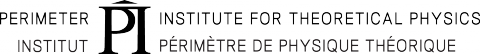
\includegraphics[width=4.3cm]{PIlogo}}
}



  \newcommand{\nc}{\newcommand}
  \newcommand{\renc}{\renewcommand}
\nc{\kos}[2]{\EuScript{K}_{#1,#2}}
\nc{\bet}{b}
\nc{\om}{\omega}
\nc{\Bn}{\mathbb{B}_n}
\newcommand{\Mirkovic}{Mirkovi\'c\xspace}
\nc{\vp}{\varphi}
\nc{\betT}{b_T}
\nc{\QT}{Q}
\nc{\HT}{S}
\nc{\ep}{\epsilon}
\nc{\Bi}{\mathbf{i}}
\nc{\BB}{B\times B}
\nc{\C}{\mathbb{C}}
\newcommand{\bT}{\mathbb{T}}
\newcommand{\bt}{\mathbbm{t}}
\newcommand{\bS}{\mathbb{S}}
\nc{\R}{\mathbb{R}}
\nc{\Cs}[1]{\underline{\C}_{#1}}
\nc{\IH}{I\!H}
\nc{\IC}{\mathbf{IC}}
\nc{\Bw}{\mathbf{w}}
\nc{\Bv}{\mathbf{v}}
\nc{\Gw}{G_w}
\nc{\up}{\vp^G_H}
\nc{\Kw}{K_w}
\nc{\cD}{\mathcal{D}}
\newcommand{\hmon}{h^{\nicefrac{-1}{n}}}
\nc{\cQ}{\mathcal{Q}}
\nc{\B}{\mathcal{B}}
\nc{\SU}[1]{\mathrm{SU}(#1)}
\nc{\SL}[1]{\mathrm{SL}(#1)}
\nc{\HU}[1]{\mathbb{H}\mathrm{U}(#1)}
\nc{\rk}{\mathrm{rk}}
\renc{\t}{\mathfrak t}
\nc{\td}{\t^*}
\nc{\g}{\mathfrak g}
\nc{\fN}{\mathfrak N}
\nc{\fS}{\mathfrak S}
\nc{\HG}{H_G}
\nc{\preO}{p\mathcal{O}}
\renc{\k}{\mathbf{k}}
\renc{\S}[1]{R_{#1}}
\nc{\Res}{\operatorname{Res}}
\nc{\Si}{\S i}
\nc{\hc}{\mathbb{H}^*}
\nc{\mc}{\mathcal}
\nc{\Hom}{\mathrm{Hom}}
\nc{\ti}{\tilde}
\newcommand{\cOg}{{\cO}^{\operatorname{g}}}
\newcommand{\cOa}{{\cO}^{\operatorname{a}}}
\nc{\cat}{\mathcal{V}}
\nc{\cata}{\mathfrak{V}}
\nc{\bla}{\underline{{\boldsymbol{\la}}}}
\nc{\hcBB}{\hc_{B\times B}}
\nc{\si}{\sigma}
\nc{\al}{\alpha}
\nc{\HH}{H\!H}
\nc{\Tor}{\mathrm{Tor}}
\nc{\KR}{\mc{KR}}
\nc{\Supp}{\mathrm{Supp}}
\nc{\ASu}{\mathrm{Supp}'}
\nc{\tri}{\tau}
\nc{\ext}{\mathrm{ext}}
\nc{\Gi}{G_{\Bi}}
\nc{\la}{\lambda}
\nc{\com}[1]{\mathcal{X}_{#1}}
\nc{\de}{\delta}
\nc{\im}{\mathrm{im}}
\nc{\fp}{\mathfrak{p}}
\nc{\fM}{\mathfrak{M}}
\nc{\fW}{\mathfrak{W}}
\nc{\A}{\mathcal{A}}
\nc{\AH}{\A_H}
\nc{\AG}{\A_G}
\nc{\Lotimes}{\stackrel{L}{\otimes}}
\nc{\be}{\beta}
\nc{\ga}{\gamma}

\newcommand{\igc}[2]
{\begin{center} \includegraphics[scale=#1]{#2} \end{center}}
\nc{\BS}[1]{G_{#1}}
\nc{\BSi}{\BS\Bi}
\nc{\excise}[1]{}
\nc{\Soer}{\mathsf{Soe}}
\nc{\Ob}{\mathrm{Ob}}
\nc{\Z}{\mathbb{Z}}
\nc{\He}{\mc H_n}
\nc{\GL}[1]{\mathrm{GL}(#1)}
\nc{\gl}[1]{\mathrm{Mat}(#1,#1)}
\nc{\F}{\underline{F}}
\newcommand{\mmod}{\operatorname{-mod}}
\nc{\spf}[1]{X_{#1}}
\nc{\en}{N}
\nc{\NC}{\mathcal{N}}
\nc{\te}{\tilde{e}}
\nc{\tf}{\tilde{f}}
\nc{\tNC}{\tilde{\NC}}
\nc{\tX}{\tilde{\mathcal{X}}}
\nc{\tY}{\tilde{\mc Y}}
\nc{\Kh}{\mathrm{Kh}}
\nc{\fg}{\mathfrak{g}}
\nc{\fG}{\mathfrak{G}}
\nc{\gr}{\operatorname{gr}}
\nc{\fb}{\mathfrak{b}}
\nc{\fh}{\mathfrak{h}}
\nc{\Fun}{\mathrm{Fun}}
\nc{\cN}{\mathcal{N}}
\nc{\Fl}{\mathfrak{B}}
\nc{\CG}{\widetilde{\C^2/\Gamma}}
\nc{\Hilb}{\mathsf{Hilb}}
\nc{\HC}{\operatorname{HC}}
\nc{\Sym}{\operatorname{Sym}}
\nc{\fQ}{\mathfrak{Q}}
\nc{\fX}{\mathfrak{X}}
\nc{\fY}{\mathfrak{Y}}
\nc{\Gr}{\mathsf{Gr}}
\nc{\cW}{\mc W}
\nc{\ft}{\mathfrak{t}}
\nc{\tU}{\mathcal{U}}
\nc{\bal}{\boldsymbol{\alpha}}
\nc{\Slod}[2]{\mathfrak{S}^{#1}_{#2}}
\nc{\Aut}{\operatorname{Aut}}
\nc{\Spec}{\operatorname{Spec}}
\nc{\Fuk}{\mathsf{Fuk}}
\nc{\modu}{\mathsf{mod}}
\nc{\mC}{\mc C}
\nc{\cL}{\mathcal L}
\nc{\cT}{\mathcal T}
\nc{\cO}{\mathscr O}
\nc{\cC}{\mathscr C}
\nc{\mD}{\mc D}
\nc{\opp}{.577350269}
\nc{\sq}{1.73205081}
\nc{\mV}{\mc V}
\nc{\BA}{\mathbf{A}}
\nc{\Br}{\mathbb{B}}
%\nc{\si}{\sigma}
\nc{\Hec}{\EuScript{H}}
\nc{\eE}{\EuScript{E}}
\nc{\eF}{\EuScript{F}}
\newcommand{\becircled}{\mathaccent "7017}
\nc{\oP}{\becircled{P}}
\nc{\Bx}{\mathbf{x}}
\nc{\BC}{\mathbf{C}}
\nc{\lag}{\langle}
\nc{\ra}{\rangle}
\nc{\K}{\mathbbm{k}}
\nc{\aff}{.4}

\DeclareMathOperator{\End}{End}
\DeclareMathOperator{\dgmod}{dg-Mod}
\DeclareMathOperator{\res}{res}
\DeclareMathOperator{\ind}{ind}

  \newtheorem{defi}{Definition}
  \newtheorem{thm}{Theorem}[section]
  \newtheorem{lem}[thm]{Lemma}
  \newtheorem{deth}[thm]{Definition/Theorem}
  \newtheorem{prop}[thm]{Proposition}
  \newtheorem{cor}[thm]{Corollary}
  \newtheorem{conj}[thm]{Conjecture}
\excise{
\newenvironment{block}
\newenvironment{frame}
\newenvironment{tikzpicture}
\newenvironment{equation*}
}

  \theoremstyle{remark}
  \newtheorem{remark}{Remark}
  \newtheorem{question}{Question}
\newcommand{\mathfig}[2]{{\hspace{-3pt}\begin{array}{c}%
  \raisebox{-2.5pt}{\includegraphics[width=#1\textwidth]{#2}}
\end{array}\hspace{-3pt}}}
\begin{document}

 \usetikzlibrary{decorations.pathreplacing,backgrounds,decorations.markings,arrows,calc,shapes.misc}
 \tikzset{knot/.style={draw=white!95!darkred,double=red,line width=2.5pt, double
     distance=1.2pt}}

\tikzset{wei/.style={draw=red,double=red!40!white,double distance=1.5pt,thin}}



\newcommand{\bfN}{\mathbf{N}}
\newcommand{\MC}{\mathfrak{M}_{\color{red}C}}
\newcommand{\MH}{\mathfrak{M}_{\color{blue}H}}
\newcommand{\knotcirc}[1]{\tikz[baseline=-2pt]{\draw[->,very thick] (0,0.3) node[above] {\scriptsize $#1$} arc (90:-315:0.3cm);}}

\begin{frame}
  \titlepage
\end{frame}
\begin{frame}
  My shameful secrets:
  \begin{itemize}
    \item<1-> I'm from the US.
    \item<2-> I've gotten old enough that I regularly make cultural references to before any of you were born.
    \item<3-> I'm a mathematician, not a physicist.
  \end{itemize}
\end{frame}
\begin{frame}
{\centerline{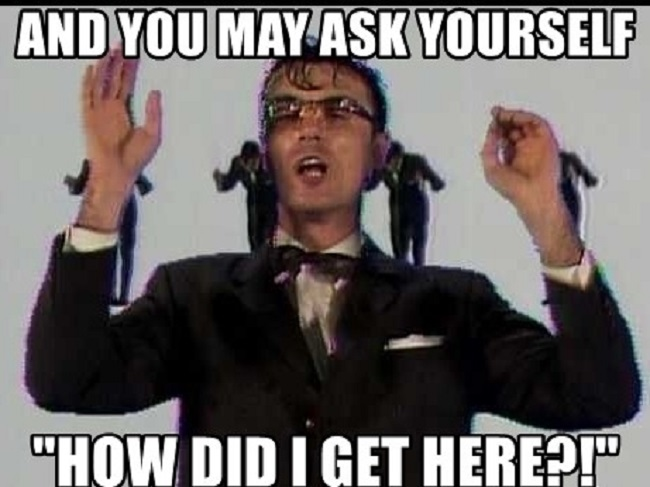
\includegraphics[width=3.5in]{./How-did-I-get-here}}}
\end{frame}

\section{Introduction}
\begin{frame}
  Physicists have a machine---path integrals, dualities, string
  theory---that outputs precise predictions about mathematical
  objects.  Predictions that mathematics cannot currently derive on
  its own.
  \begin{block}{}
    Dualities especially create ``secret passages'' between parts of
    mathematics with little obvious connection.
  \end{block}
  Many of these predictions say: {\it two things mathematicians
    defined independently, for totally different reasons, are
    secretly the same.}
  \pause
  \bigskip

  My research: take such a prediction and build the mathematics
  needed to prove it.  The proof is never a formality---it usually
  requires new structures, and those structures often say something
  back to the physics.
  \bigskip

  (I won't compute a cross-section for you.  But if you want to know
  what your QFT is doing to {\it mathematics}, that's my department.)
\end{frame}

\section{Higgs and Coulomb branches}
\begin{frame}
  Start with a 3d gauge theory $\mathcal{T}(G,N)$: a compact group
  $G_c$ acting on a complex representation $N$, and the induced
  $\sigma$-model into $T^*N\cong \mathbb{H}\otimes_{\C} N$.  This
  theory has $\mathcal{N}=4$ supersymmetry.
  \begin{block}{}
    With this much SUSY, there are two topological twists
    $Q_{\color{red} A}$ and $Q_{\color{blue} B}$.
  \end{block}
  In a twisted 3d theory, the local operators form a {\bf commutative
    algebra} with a {\bf Poisson bracket} (the secondary product): the
  functions on the moduli space of vacua.
  \bigskip

  Two twists $\Rightarrow$ two Poisson varieties:
  \[\MH=\Spec Z_{\color{blue} B}(S^2) \qquad \MC=\Spec Z_{\color{red}
      A}(S^2)\]
  the {\bf \color{blue} Higgs} and {\bf \color{red} Coulomb} branches.
\end{frame}

\begin{frame}
  The two branches are not created equal:
  \begin{itemize}
  \item $\MH$ is classical: the hyperk\"ahler quotient
    $\mathbb{H}^n/\!/\!/\!/G_c$ (Hitchin--Karlhede--Lindstr\"om--Ro\v
    cek, 1987).  Mathematicians digested this decades ago.
  \item $\MC$ receives quantum corrections from monopoles.  For
    $\sim$20 years, physicists computed examples of a space with {\bf
      no mathematical definition}.
  \end{itemize}
  \begin{block}{}
    Braverman--Finkelberg--Nakajima (2016): a rigorous definition,
    via a convolution algebra built from a moduli space of monopoles.
    New mathematics, forced into existence by physics.
  \end{block}
  Example: $G=U(1)$ acting on $N=\C^n$ gives
  $\MC\cong\C^2/\Z_n$.\bigskip

  These spaces include the nilcones of semisimple Lie algebras, and
  behave like a new class of ``semisimple Lie algebras,'' vastly
  generalizing the Killing classification.
\end{frame}

\section{Duality}
\begin{frame}
  {\bf 3d mirror symmetry} (Intriligator--Seiberg, 1996): pairs of
  theories $\mathcal{T},\mathcal{T}^!$ equivalent in a way that swaps
  $Q_{\color{red} A}\leftrightarrow Q_{\color{blue} B}$.  In
  particular:
  \[\MH(\mathcal{T})\cong \MC(\mathcal{T}^!)\qquad
    \MC(\mathcal{T})\cong \MH(\mathcal{T}^!)\]
  To a physicist: a duality.  To a mathematician: an outrageous list
  of conjectures pairing spaces with no visible relationship---one
  that generalizes the Langlands duality of semisimple Lie algebras.
  \begin{block}{Theorem (Braden--Licata--Proudfoot--W.)}
    For many such dual pairs, the categories $\mathcal{O}$---categories of
    representations tailored to the geometry of the two
    branches---are Koszul dual.
  \end{block}
  Representation theory on one side determines representation theory
  on the other.  The physicists consider this obvious; the proof is
  $\sim$200 pages.  Physics is fast, and theorems are slow---but the
  theorems are what make the next round of predictions checkable.
\end{frame}

\begin{frame}
  Where this thread is now:
  \begin{itemize}
  \item {\bf Functoriality:} gauging on the physics side becomes a
    Hamiltonian reduction operation between Coulomb branches; this
    proves, e.g., that $\overline{T^*(G/U)}$ for $\SL{n}$ is a Coulomb
    branch (conjecture of Bourget et al.).
  \item {\bf Coherent sheaves:} explicit quiver-style descriptions of
    the categories of sheaves on resolved Coulomb branches---in
    physics language, the categories of boundary conditions.
  \end{itemize}
  \begin{block}{}
    These categories are exactly what is needed to make Aganagi\'c's
    string-theoretic knot homology into algebra.
  \end{block}
  \centerline{\ldots which brings me to knots.}
\end{frame}

\section{Knots and the planar limit}
\begin{frame}
  Witten (1989): expectation values of Wilson loops in Chern--Simons
  theory are knot invariants; $\SU2$ with the fundamental
  representation gives the Jones polynomial.

  \vspace{1in}
  % picture: a knot (trefoil?) drawn as a Wilson loop in a solid ball,
  % maybe with the CS action floating next to it

  Coloring a knot $K$ by $\bigwedge^{\!m}\C^N$ for all $m,N$ packages
  into the two-variable {\bf HOMFLYPT polynomial}: a function of $q$
  and $g=q^N$.  For fixed $K$, these satisfy recursion relations in
  the coloring $m$: the ``deformed $\hat{A}$-polynomial.''
  \bigskip

  Physics question ('t Hooft): what happens in the planar limit?
  \[N\to\infty,\qquad q\to 1,\qquad g=q^N \text{ fixed}\]
\end{frame}

\begin{frame}
  Gopakumar--Vafa: large-$N$ Chern--Simons on $S^3$ is a topological
  string on the resolved conifold.  A knot adds a brane on its
  conormal Lagrangian $L_K$.
  \bigskip

  The brane has its own invariant: {\bf knot contact homology}
  and its augmentation variety (Ekholm, Ng, \ldots)---defined by
  counting holomorphic curves, with no reference to Chern--Simons
  whatsoever.
  \begin{block}{Prediction (Aganagi\'c--Vafa)}
    The augmentation variety of $K$ is the classical limit of the
    recursion relations satisfied by its HOMFLYPT polynomials.
  \end{block}
  Two objects, two communities, no known map between them.  This is
  exactly the pattern from the start of the talk.
\end{frame}

\begin{frame}
  Idea (after Gaiotto--Kannagi--Sanjurjo): treat the coloring $m$ as a
  {\bf formal variable}.  Then $\mu=q^m$ and the shift
  $\la\colon m\mapsto m-1$ generate a quantum torus,
  $\la\mu=q\mu\la$, acting on a module built from skein theory: the
  {\bf HOMFLYPT difference module}.
  \bigskip

  One honest calculation.  The MOY relations give, for the unknot:
  \[\knotcirc{m} \;=\;
    \frac{q^{N-m+1}-q^{-N+m-1}}{q^{m}-q^{-m}}\;\knotcirc{m-1}\]
  Substituting $g=q^N$, $\mu=q^m$ (no $N$, no $m$!):
  \[\knotcirc{m}\;=\;\frac{qg\mu^{-1}-q^{-1}g^{-1}\mu}{\mu-\mu^{-1}}\,
    \la\;\knotcirc{m}\]
  So $\mu-\mu^{-1}-\la\,(qg\mu^{-1}-q^{-1}g^{-1}\mu)$ annihilates the
  unknot: its deformed $\hat{A}$-polynomial, with no computation of
  any knot invariant.
\end{frame}

\begin{frame}
  \begin{block}{Theorem (W.--Zaimi, 2026)}
    At $q=1$, the HOMFLYPT difference module {\bf is} the degree-0
    abelianized knot contact homology of $K$.
  \end{block}
  \begin{itemize}
  \item This does not fully prove Aganagi\'c--Vafa, but reduces it to
    sharply stated algebra conjectures (injectivity of an evaluation
    map).  Here is exactly what remains.
  \item The proof is purely algebraic: diagram calculus.  No
    holomorphic curves, no path integrals.  Elementary tools,
    non-elementary conclusion.
  \end{itemize}
  This paper owes a large debt to conversations with Davide
  Gaiotto---the kind of accident that only happens in this building.
\end{frame}

\section{Coda}
\begin{frame}
  The same shape, twice:
  \begin{itemize}
  \item Physics predicted equalities between independently defined
    objects: Higgs $\leftrightarrow$ Coulomb; recursions
    $\leftrightarrow$ augmentation varieties.
  \item Proving them required inventing structures---BFN construction,
    symplectic duality, difference modules---that now have lives of
    their own.
  \end{itemize}
  \begin{block}{}
    And the machine keeps producing: Aganagi\'c predicts knot
    homologies for $\mathfrak{gl}(m|n)$---$\mathcal{N}=2$ physics,
    matrix factorizations---with no mathematical construction yet.
  \end{block}
  The mathematics involved is learnable: the planar-limit proof runs
  on a diagram calculus you could pick up in weeks, not years.
  \bigskip

  Physics is decades ahead of the proofs.  Catching up is a full-time
  job, with room for help.
\end{frame}

\excise{
%% Spare parts: one more frontier flavor for the ``where this thread
%% is now'' frame, if pace allows.  Both name-drop well at PI; neither
%% gets more than a sentence.
\begin{frame}
  \begin{itemize}
  \item Costello--Creutzig--Gaiotto: the Coulomb branch can be
    recovered from a vertex operator algebra built on the Higgs
    branch---the only known passage from Higgs to Coulomb that
    doesn't route through the full QFT.
  \item Quantum Hikita (with Gaiotto et al.): twisted traces of a
    quantization of $\MH$ match the quantum cohomology of the mirror
    $\MC$.
  \end{itemize}
\end{frame}
}

\end{document}
